\documentclass[english,a4paper,12pt]{article}
\usepackage[utf8]{inputenc} %for å bruke æøå
\usepackage{babel}
\usepackage{verbatim} %for å inkludere filer med tegn LaTeX ikke liker
\usepackage[document]{ragged2e}
\bibliographystyle{plain}
\usepackage{amsmath}
\usepackage{ulem}
\usepackage[pdftex]{graphicx}
\usepackage{gensymb}
\usepackage{float}
\usepackage{hyperref}
\usepackage{amssymb}
\usepackage[top=0.6in, bottom=0.8in, left=0.9in, right=0.7in]{geometry}
\usepackage{listings}
\usepackage{color}
\usepackage{tikz}

\usepackage{filecontents}
\begin{filecontents}{mybib.bib}
@book{Turbulence,
   author    = "William K. George
Department of Aeronautics
Imperial College of London
London, UK
and
Professor of Turbulence Emeritus
Department of Applied Mechanics
Chalmers University of Technology
Gothenburg, Sweden",
   title     = "Lectures in Turbulence for the 21st Century",
   publisher = "",
   address   = "\url{}",
   pages   = "247--288",
   year      = "2013"
}

@unpublished{SoundofTurbulence,
   title     = "The sound of turbulence",
   author = "Lily Xu at Department of Mathematics
Faculty of Mathematics and Natural
Sciences
University of Oslo",
   note   = "\url{https://www.google.no/url?sa=t&rct=j&q=&esrc=s&source=web&cd=1&ved=0ahUKEwicndmvh-PTAhWoNJoKHdZ1A-8QFggpMAA&url=https%3A%2F%2Fwww.duo.uio.no%2Fbitstream%2Fhandle%2F10852%2F45389%2FThesis_Lily_Xu.pdf%3Fsequence%3D1&usg=AFQjCNF0bezoP5hYeMiMHhQcyxQqw8JG3Q}"
}

\end{filecontents}

\usepackage{natbib}
\usepackage{bibentry}
\nobibliography*

\title{LabView project - MEK4600}
\author{Shako Farhad, Valentyna Pysarieva \& Farnaz Rezvany}
\date{\today}

\begin{document}

\definecolor{codegreen}{rgb}{0,0.6,0}
\definecolor{codegray}{rgb}{0.5,0.5,0.5}
\definecolor{codepurple}{rgb}{0.58,0,0.82}
\definecolor{backcolour}{rgb}{0.95,0.95,0.92}
 
\lstdefinestyle{mystyle}{
    backgroundcolor=\color{backcolour},   
    commentstyle=\color{codegreen},
    keywordstyle=\color{magenta},
    numberstyle=\tiny\color{codegray},
    stringstyle=\color{codepurple},
    basicstyle=\footnotesize,
    breakatwhitespace=false,         
    breaklines=true,                 
    captionpos=b,                    
    keepspaces=true,                 
    numbers=left,                    
    numbersep=5pt,                  
    showspaces=false,                
    showstringspaces=false,
    showtabs=false,                  
    tabsize=2
}
 
\lstset{style=mystyle}

\maketitle

\begin{abstract}
With ever increasing computational power, we get more and more numerical data on turbulence, but at the same time there is a lack of experimental data on turbulence. We examined turbulence of water flowing through a plastic tube by capturing the sound waves emitted with a microphone. \\
Our experiments were set up in the following manner; water flows down from a tank, through a tube and a microphone picks up the flow sound. The sound signals from the microphone went through an amplifier and then the DAQ wrote the signals to a file that was stored on the computer. By adjusting the height of the water tank we strove to reach certain Reynold numbers, $50$, $500$, $2000$ and $4000$. \\
The higher the Reynolds number, the higher the energy output is. At the same time the data was contaminated with noise. Because of this, our findings may be inconclusive.

\end{abstract}

\section*{Introduction}
Turbulence is ever present in the air we breathe, the water we drink, the clouds above us, the blood that flows through our veins, and much more. The exploration of turbulence is important to understand all these integral mechanism in our lives \cite{Turbulence}. We will examine how sound from flowing water can be used to say something about the turbulence in said water.\bigskip

Trying to measure turbulence by only using sound waves from the flowing water is something that has been tried many times before, but the results has shown varying degrees of success. The limitations are many and they usually come down to the lack of adequate equipment. But despite this, Lily Xu \cite{SoundofTurbulence}, a master student at UiO, had used similar methods to us to measure turbulence in hopes to fight aneurysms that can cause strokes and sudden deaths. \bigskip 

In our efforts we taped a microphone to a tube that had water flowing through with different Reynolds numbers, 50, 500, 2000 and 4000. While we did observe that higher Reynolds numbers resulted in a higher mean energy output in the frequency spectra plots, we also saw that the data was easily corrupted by noise.

\section*{Theoretical models and methods}
We wrote a program in LabView that read sound signals from a microphone and both wrote those signals to a file in the 'lvm' format. The sound signals from the microphone went through an amplifier and then the DAQ wrote the signals to a file that was stored on the computer. It was made sure that the signal from the amplifier to the DAQ was between $\pm 10$ V, to avoid the signal from being truncated at the lower and upper ends. \bigskip 

In LabView we could also set the amount of samples to read each time. This meant that the DAQ would store a vector of specific length with values before calling the CPU to write the contents of that vector to the hardrive on the computer. It was important to not have a too long vector, as it may fill up the local memory of the DAQ. It was also important to not have a too short vector, because it would make very many calls to the CPU to write to the hardrive. This would lead to high CPU usage and heat output, and slowdowns in other programs. We chose the vector length to be $2^{11} = 2048$. A multiple of $2$ makes better use of the local memory of the DAQ, and a vector length of $2048$ made sure that the DAQ did not overload the CPU with write calls. \bigskip

We chose the sampling frequency to be $20000$ Hz because we believed that the highest signal frequency would be at around $8000$ Hz. From the Nyquist-Shannon sampling theorem we knew that we had to select a sampling frequency that was two times the highest signal frequency. And because we wanted to avoid loss of data from inadequate sampling frequency, we added another $4000$ Hz, giving us a total of $20000$ Hz. \bigskip

The experiment was setup as seen in figure \ref{fig:1}. The water flows down from the white tank, through a tube on the table, behind the laptop, and before it flows in to the blue bucket at the bottom right, the microphone picks up the flow sound. The blue bucket is placed on top of a digital flat scale, measuring in grams. The height of the white tank was measured from the water surface to the floor with a digital laser device, and then subtracted that height with the height from the tube end to the floor, which was about 0.47 m. We were supposed to reach certain Reynold numbers (50, 500 2000 and 4000) by adjusting the height of the white water tank. \bigskip


The Reynolds number is given by:

$$\text{Re} = \frac{\rho \cdot v \cdot d}{\mu},$$

where $\rho \approx 998.2$ kg/m$^3$ is the water density, $v$ is the water velocity, $d = 0.0079$ m is the inner diameter of the tube, and $\mu = 0.001002 \text{ Pa} \cdot \text{s}$ is the dynamic viscosity. \smallskip

To calculate the velocity, $v$, we used the formula $v=\frac{V}{t\cdot A}$, where $V$ is the volume, $t$ is the time passed, and $A$ is the cross sectional area of the tube. We have $A=\pi \cdot r^2$ and $V=\frac{\text{mass}}{\rho}$. We already knew the mass from the digital scale underneath the blue bucket, and we let the water flow for five minutes every time. In table \ref{tab:1} we can see the calculated values from the different experiments.

\begin{table}[h!]
    \centering
    \begin{tabular}{|c|c|c|c|c|}\hline
    Reynolds number & Velocity [m/s] & Height [m] & Mass [kg] & Time [s] \\ \hline
    52.0075 & 0.0066 & 0.1620 & 0.0970 & 300\\ \hline
    512.0324 & 0.0651 & 0.3740 & 0.9550 & 300\\ \hline
    1940.3614 & 0.2466 & 1.0200 & 3.6190 & 300\\ \hline
    3728.9897 & 0.4738 & 2.6700 & 6.9550 & 300\\ \hline
    \end{tabular}
    \caption{Data from four different experiments where the white tank was placed at different heights.}
    \label{tab:1}
\end{table}

\begin{figure}[H]
    \centering
    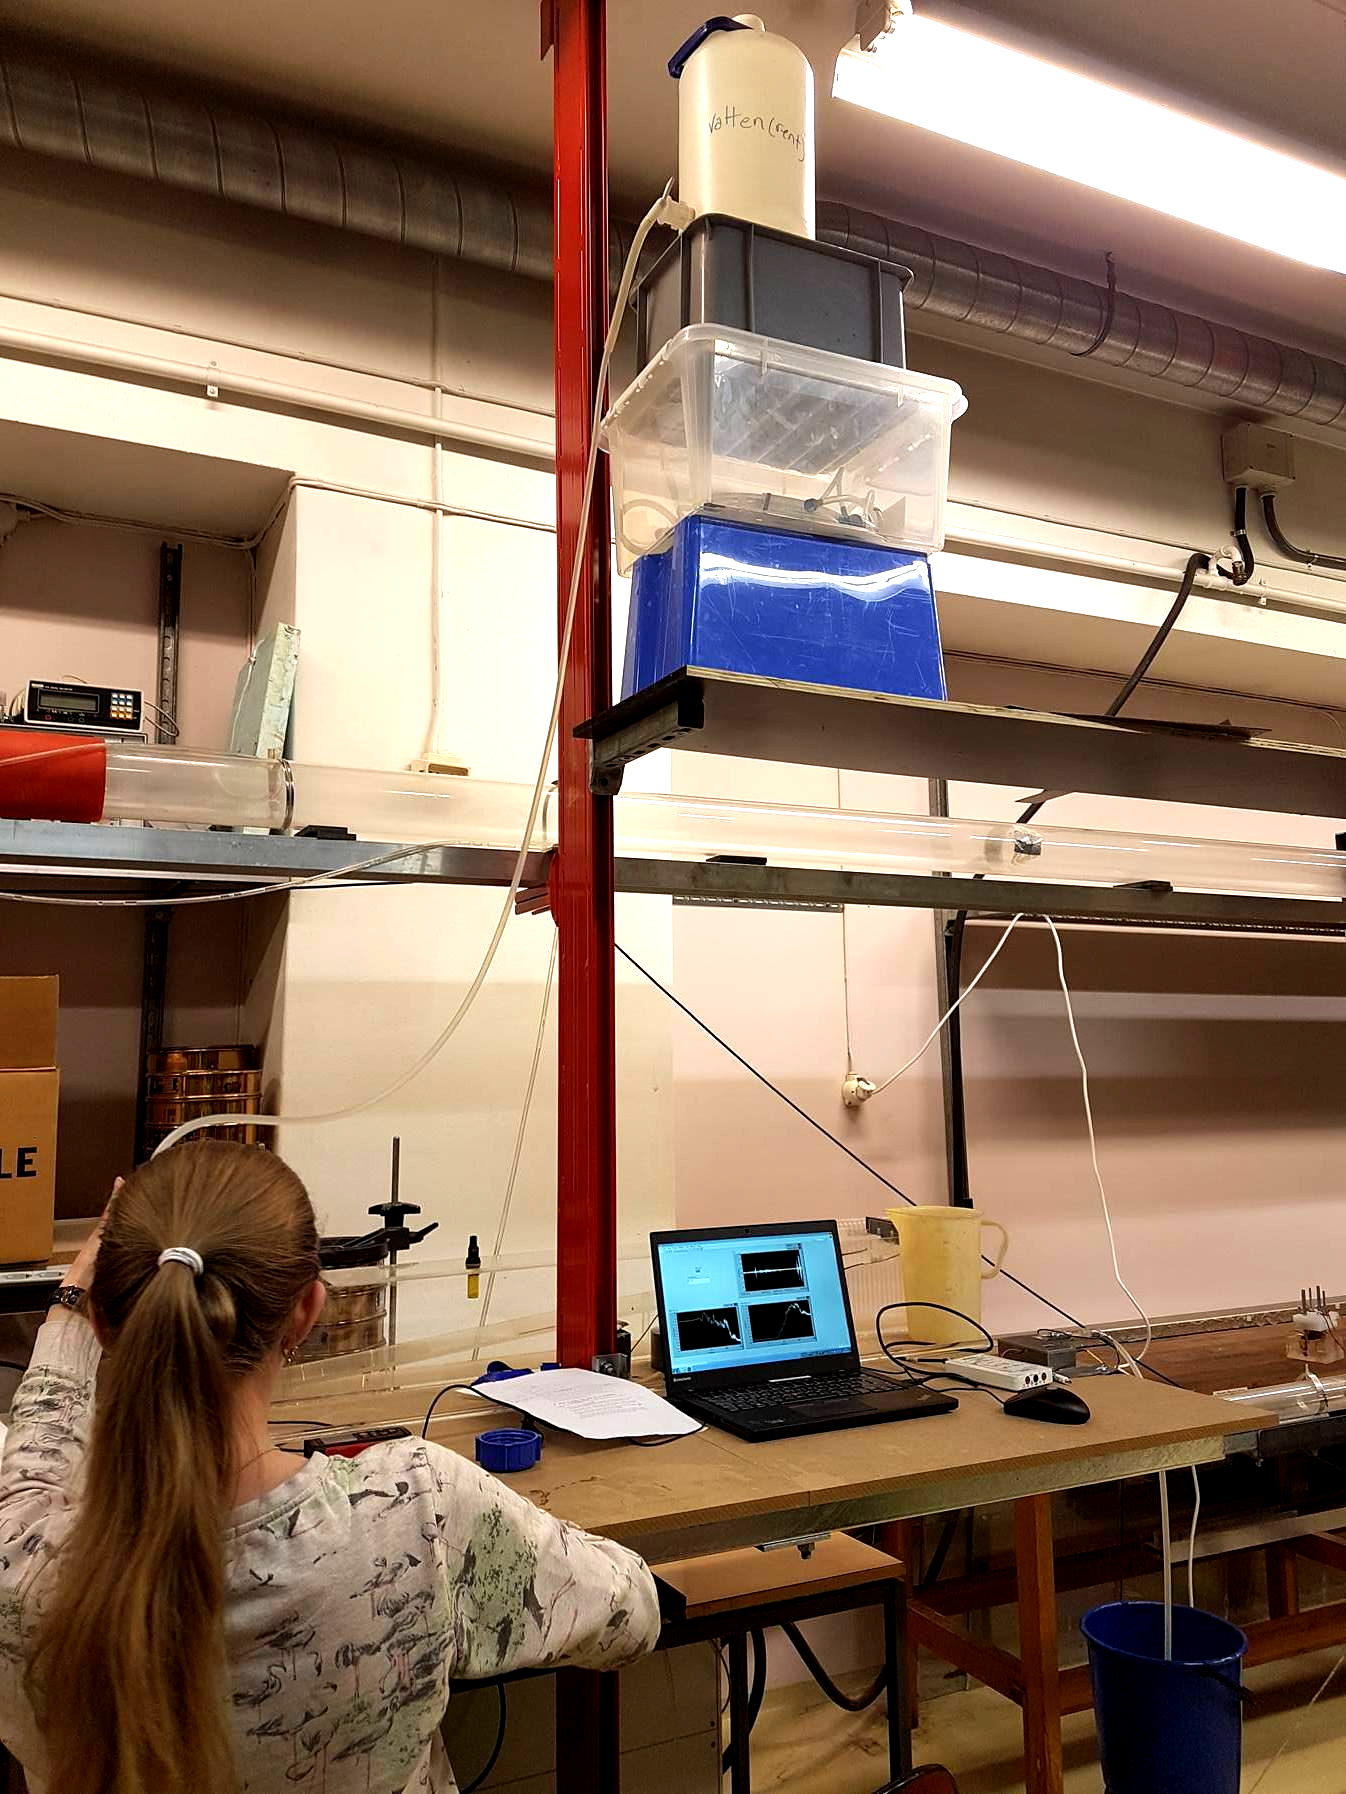
\includegraphics[width=150mm]{ExperimentSetup.png}
    \caption{The setup of the experiments. The white tank at the top contains water that flows through the tube down into the blue bucket. The flow sound signals are measured with a microphone that is amplified and stored on the laptop with the white DAQ box. The water flow was controlled with a valve that was positioned on the table in front of the girl.}
    \label{fig:1}
\end{figure}

\section*{Results}

\begin{figure}[H]
    \centering
    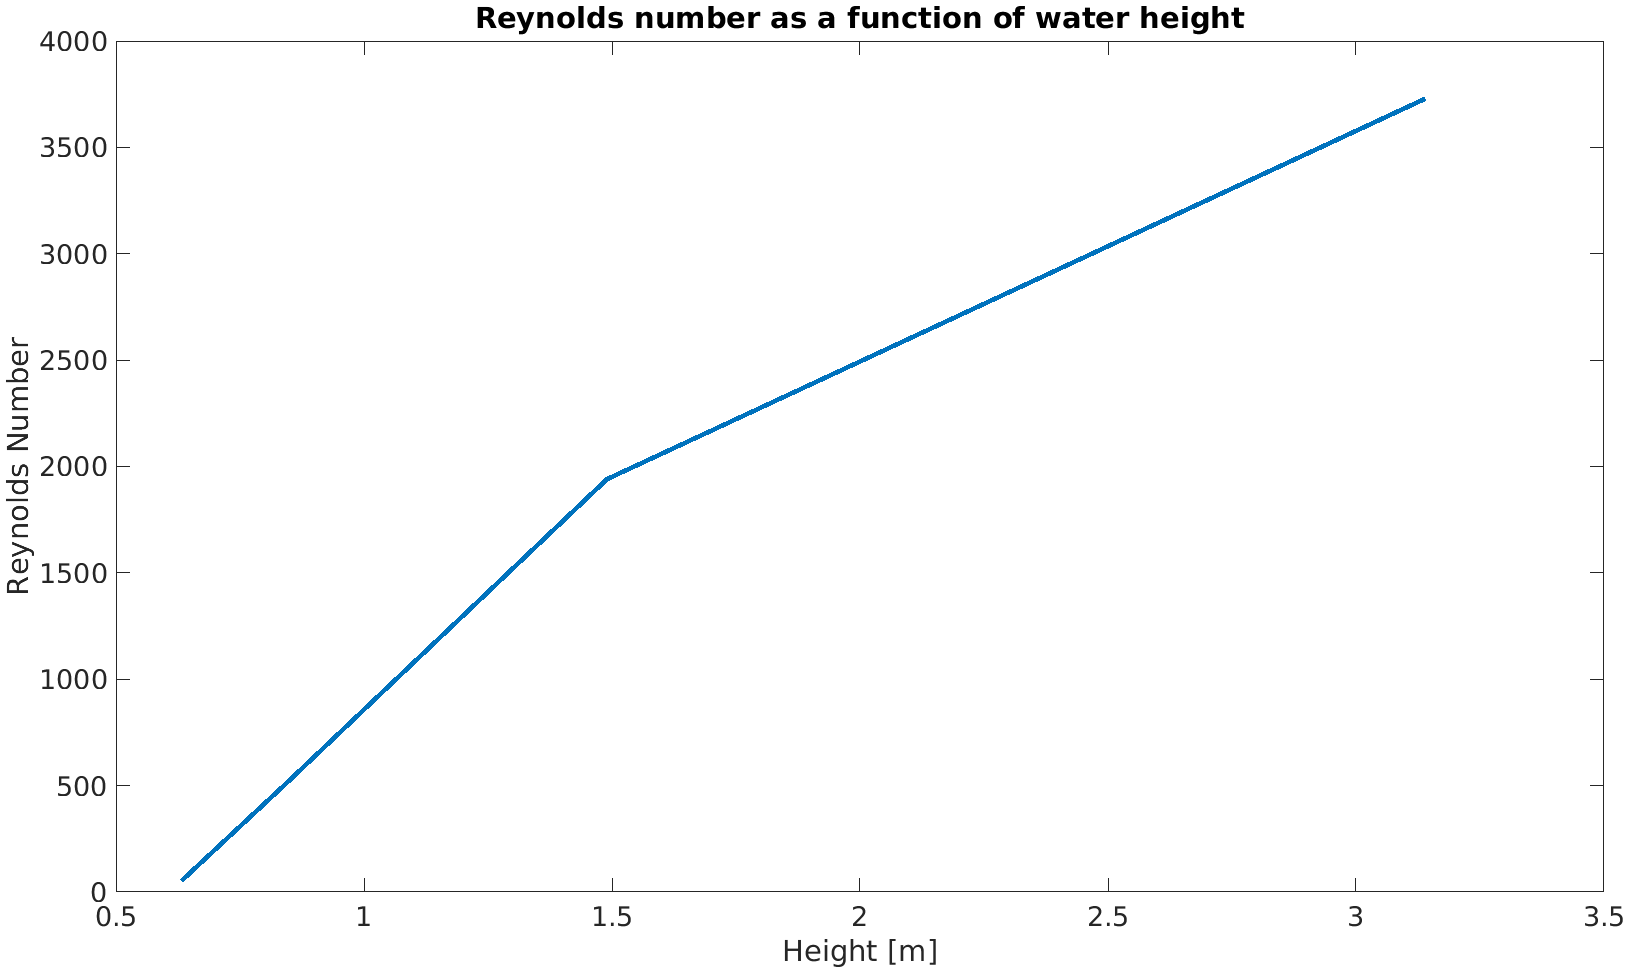
\includegraphics[width=170mm]{ReVsHeightPlot.png}
    \caption{Diminishing returns are starting to be visible already at $1$ m height. More data points are needed.}
    \label{fig:2}
\end{figure}

\begin{figure}[H]
    \centering
    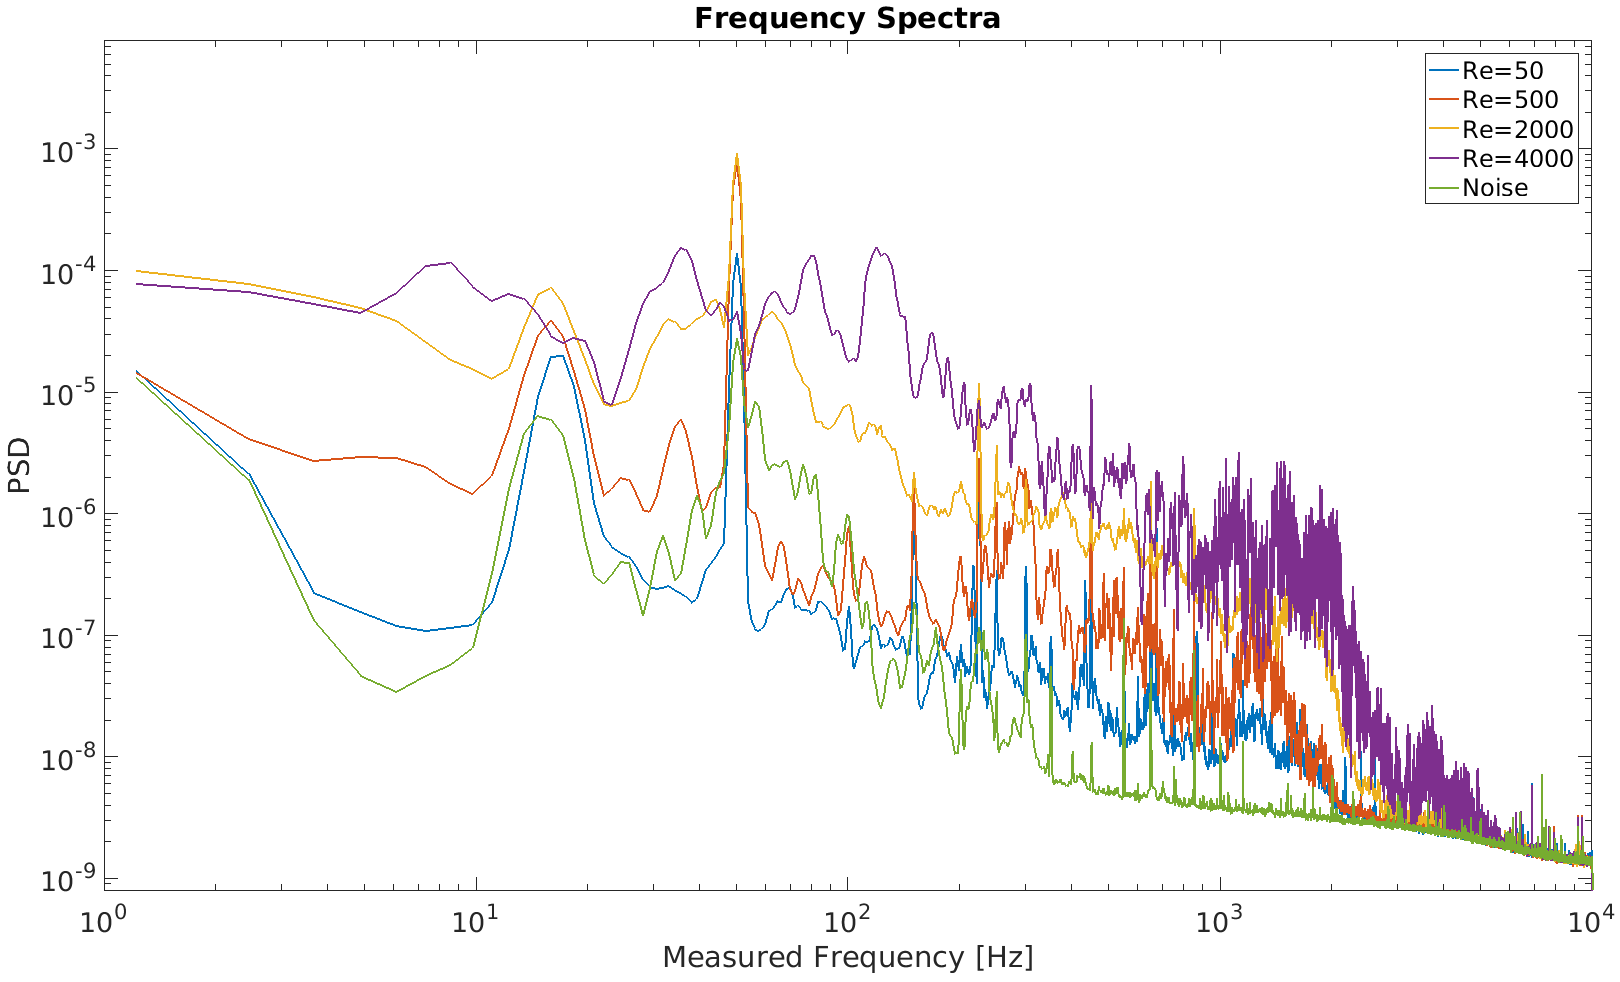
\includegraphics[width=170mm]{FrequencySpectraPlot.png}
    \caption{The frequency spectra of the different experiments and background noise. The higher the Reynolds number is, the higher energy output. Especially in the high frequency range, we can see the effect of higher Reynolds number clearly.}
    \label{fig:3}
\end{figure}

\begin{figure}[H]
    \centering
    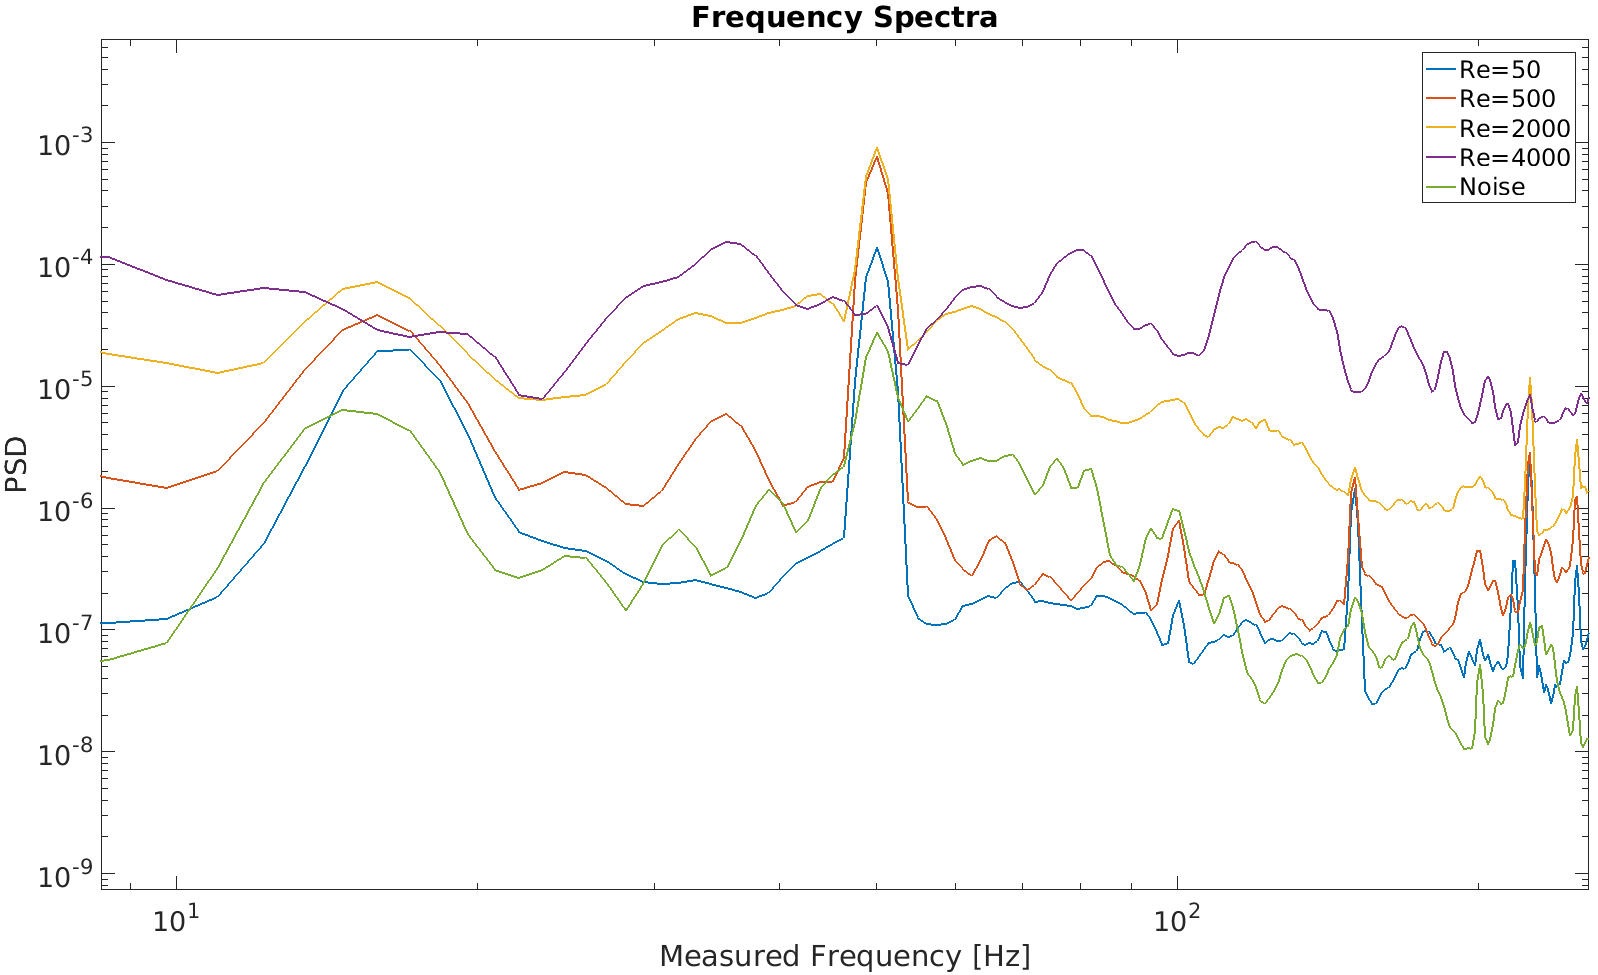
\includegraphics[width=170mm]{FrequencySpectraPlotZoomed.png}
    \caption{The same frequency spectra as in figure \ref{fig:3}, but here we focus on frequency between $10$ to $200$ Hz. The clear trend of higher energy output for higher Reynolds number is not as prominent here. For Re=4000 we get lower energy output than Re=50 and re=500 around $60$ Hz.}
    \label{fig:4}
\end{figure}

\begin{figure}[H]
    \centering
    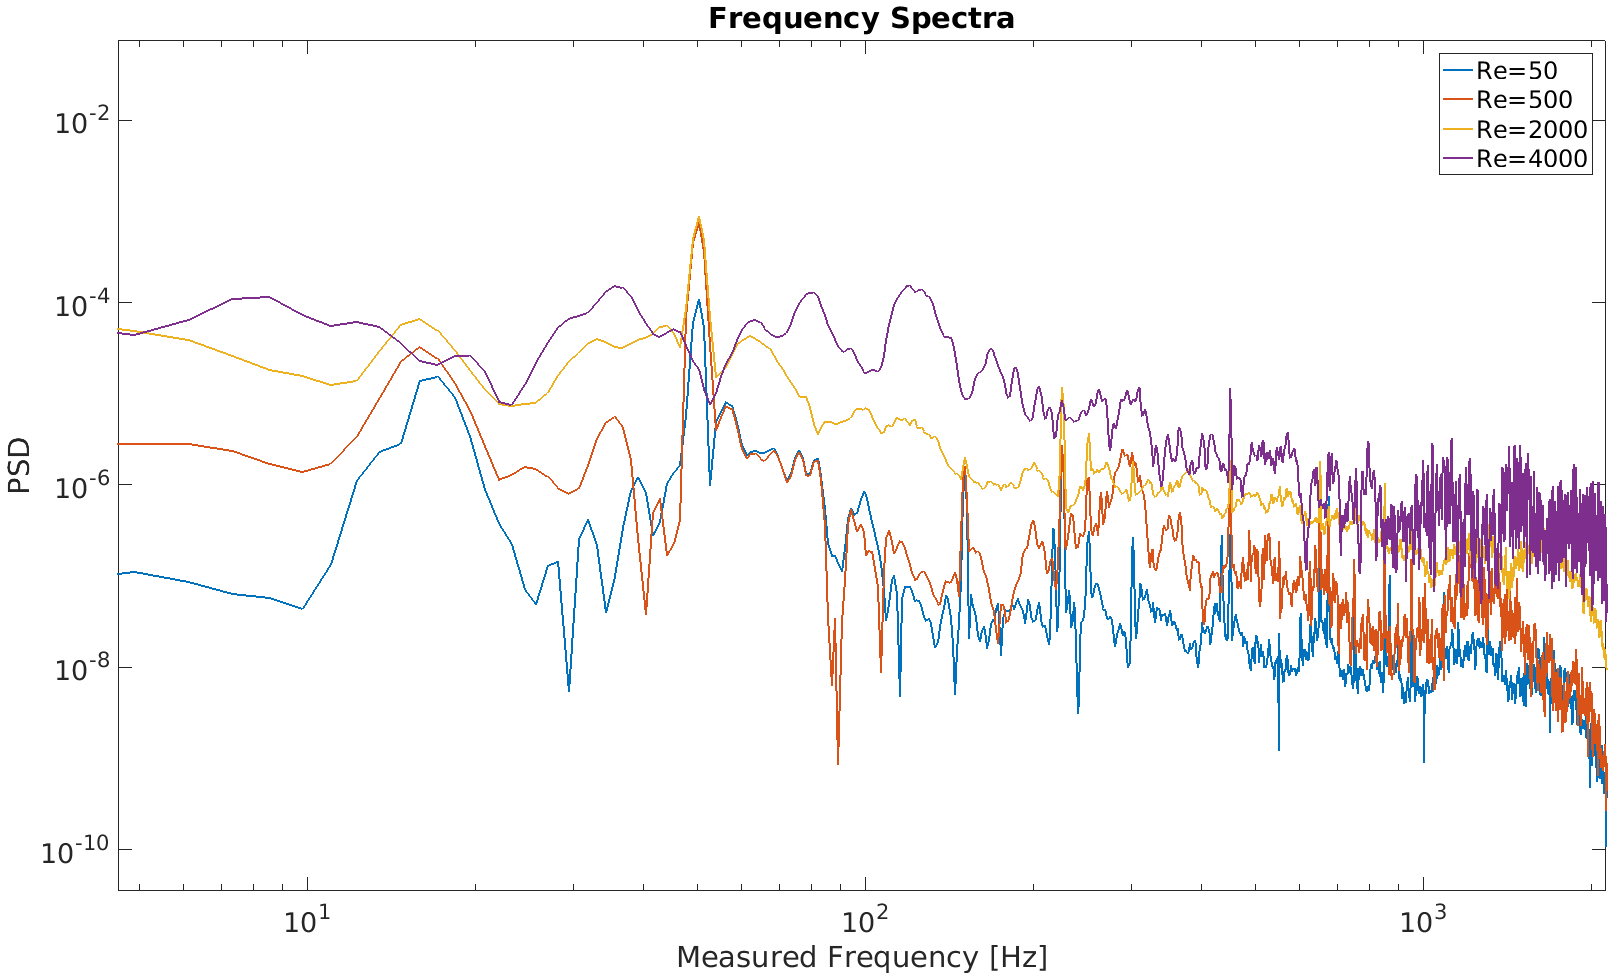
\includegraphics[width=170mm]{FrequencySpectraPlotWithoutNoise.png}
    \caption{The noise has been subtracted from the other Power Spectra Density plots. We see that the noise did not alter the peak at around 145 Hz, but that there are dramatic reductions at some specific points like at 120 Hz.}
    \label{fig:5}
\end{figure}

\begin{figure}[H]
    \centering
    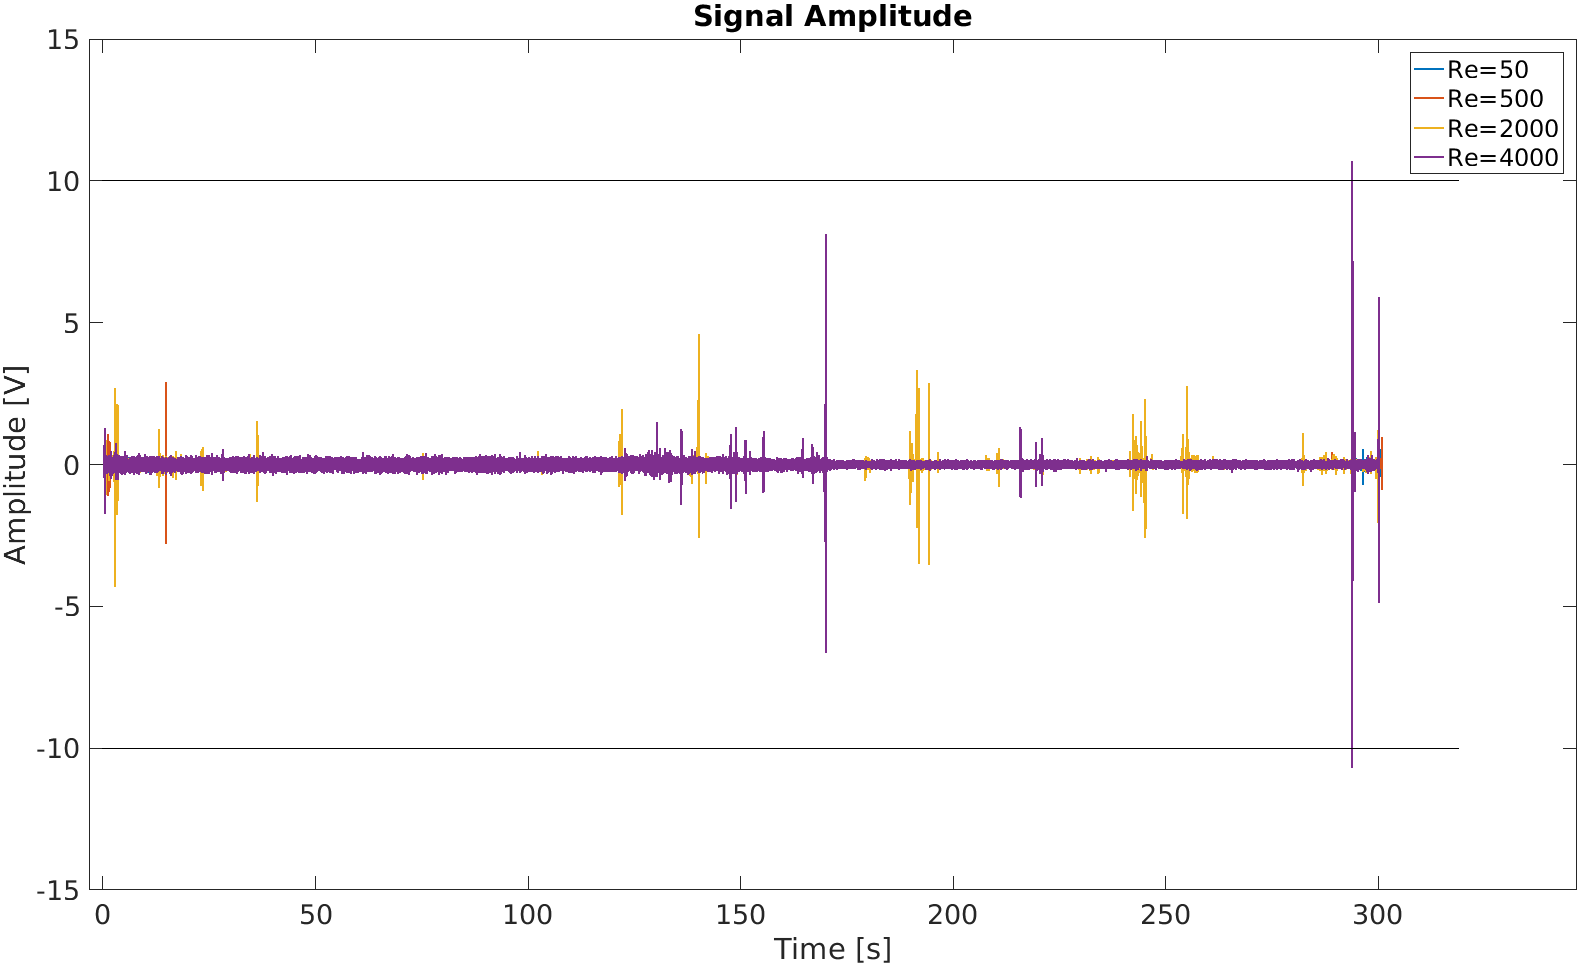
\includegraphics[width=170mm]{SignalAmplitude.png}
    \caption{Here we can see that all the measurements were within $\pm 10$ V, apart from a specific point at the end of the run. There we can see that the run for Reynolds number 4000 has registered above 10 V and below -10 V.}
    \label{fig:6}
\end{figure}

\section*{Discussion}
The setup of the experiment was very interesting and enjoyable. Navigating LabView is sometimes a bit unintuitive, but despite that, we did setup the LabView program reasonably quick. The challenge was to figure out how to calculate the Reynolds number with the setup as seen in figure \ref{fig:1}. \bigskip

After understanding and applying the theory, we met with the unfortunate reality of noise contamination. There were many others at the laboratory and they were all working on their own projects and experiments. This resulted in noise to the microphone that was not easily filtered or reduced. But even if the laboratory was empty, we still would have noise from the different vents, lights, us, etc. Also the sound waves coming from the water in the tube will be dampened by the thickness of the tube. This adds another layer of noise to the data. For Reynolds number 50 and 4000 we used the valve to control the water flow, by not having it completely open, to get the right Reynolds number. This causes turbulence and noise as well. \bigskip

We wanted to filter out noise from the data, but it was difficult to ascertain what frequency ranges needed to be filtered out. From the frequency spectra of the background noise in figure \ref{fig:3}, we ascertained that the noise had to be in the range between $100$ Hz and $250$ Hz. We were told that this was completely wrong by professor Atle Jensen, as the interesting frequency range was exactly that. Therefore we concluded that filtering the noise from the raw data would potentially remove frequencies that would have unintentional consequences on the results. \bigskip

One curious artifact is that the data for Re=4000 in figure \ref{fig:6} has a spike that goes above 10 V and below -10 V. This should be impossible as the DAQ should have truncated that to 10 V and -10 V. This may be the reason to why we see Re=4000 have a lower energy output in \ref{fig:4} at around 145 Hz. \bigskip

From figure \ref{fig:6} we can see that if we look away from the big spikes, the data is all contained within -1 to 1 V. This is acceptable, but with a better microphone and perhaps a better amplifier, we could use the range of the DAQ better. Using more of the -10 to 10 V range of the DAQ would give more precise readings. \bigskip

The very fact that we can make some observations at all like in figure \ref{fig:3} despite the noise is very fortunate. Then again, the noise had given us curious artifacts like in figure \ref{fig:4}, which makes our findings inconclusive.\bigskip

One inconsequential, but interesting finding is shown in figure \ref{fig:2}. Here we can see that the Reynolds number as a function of water height is shaped like the log function. Perhaps with more data, we could see this log function more clearly, and if that is the case, at what point does it take a great amount of height, for the Reynolds number to increase significantly? \bigskip

For further experimentation of measuring turbulence with a microphone, we need to be more diligent with noise reduction. Preferably the experiments should be carried out in a soundproof room, with a more powerful microphone. Also, if possible, the microphone should be placed on the inside of the tube, such that the sound waves are not dampened by the tube.

\section*{Conclusion}
From figure \ref{fig:3} we can clearly see that higher Reynolds numbers create more energy, and also that this energy is more prominent in the high frequency range. At the same time, we can see that our findings may be inconclusive because of noise contamination, as seen in figure \ref{fig:4}. \bigskip

We subtracted the noise seen in figure \ref{fig:3} from all the other PSD plots and plotted the result in figure \ref{fig:5}. We can see that the overall trends do not change, but that especially the spike at around 145 Hz is unchanged even after directly subtracting by the noise. This could of course be because the noise is about 10 times lower in magnitude and therefore makes little difference when subtracting the other PSDs from it. 

\section*{Appendix}
Visit the below link to see the matlab codes, the LabView files, and plots and images.

\url{https://github.com/ShakoFarhad/LabView-Project-MEK4600}

\bibliographystyle{plainnat}
\bibliography{mybib} \bigskip \bigskip
\end{document}
